\documentclass[sigconf]{acmart}
\usepackage{graphicx}
\usepackage{graphicx}
\usepackage{hyperref}
\usepackage{todonotes}

\usepackage{endfloat}
\renewcommand{\efloatseparator}{\mbox{}} % no new page between figures

\usepackage{booktabs} % For formal tables

\settopmatter{printacmref=false} % Removes citation information below abstract
\renewcommand\footnotetextcopyrightpermission[1]{} % removes footnote with conference information in first column
\pagestyle{plain} % removes running headers

\newcommand{\TODO}[1]{\todo[inline]{#1}}
\graphicspath{{images/}}
\begin{document}
\title{Big Data and the Customer Experience Journey}


\author{Ashley Miller}
\orcid{HID329}
\affiliation{%
  \institution{Indiana University}
  \date{December 2017}
}
\email{admille@iu.edu}



% The default list of authors is too long for headers}
\renewcommand{\shortauthors}{G. v. Laszewski}


\begin{abstract}
A customer's experience journey consists of multiple touchpoints along the way as they make choices in which companies and brands to interact with and ultimately, purchasing decisions. While the customer experience journey may differ based on product, service, audience, time, as well as a company's capabilities and strategic initiatives, the need to understand the customer transcends all industries. These touchpoints are increasingly moving to the digital space through online search, mobile interaction, social media, email, in addition to other methods that may not even be in existence as of yet. Given the number of these touchpoints across customers and the ability to track customers across multiple methods, understanding the experience of customers through the use of big data provides opportunities for companies to better enhance the customer experience journey. Real-time recommendations, personalized marketing messages, and geo-targeted advertising can all play a role in \textit{nudging} the customer appropriately when companies are looking to drive customer interaction and behavior. We will seek to explore this customer experience journey in the digital environment and introduce relevant case studies where companies and industries have started to utilize big data and analytics to better understand and customize the customer experience journey through digital efforts.
\end{abstract}

\keywords{i523, hid329, big data, analytics, customer experience journey, consumer behavior, digital marketing}

\maketitle
\section{Introduction}
The customer experience journey has been largely explored from a psychological and behavioral standpoint \cite{Stoicescu2015}. Dating back to the near 1800s, marginal and expected utility of actions were detailed by Nicholas Bernoulli, among others, to better understand how purchasing decisions were made \cite{Stoicescu2015}. From related work that followed in this field of studying behavioral economics, research has shown that purchasing decisions are not linear and at times, are not even rational as cognitive, emotional, and social factors can all play a role into how a customer makes a purchasing decision \cite{Stoicescu2015}. As described by Stoicescu, the reason why researchers started to study purchasing behavior was due to the ``diversification of need" \cite{Stoicescu2015}. 

However, with diversification also comes complexity. The more choices a customer is given, the harder it can become for them to make a decision \cite{Stoicescu2015}. With every product choice, there also is an opportunity for interaction or \textit{touchpoints} along this customer experience journey \cite{Meyer2007}. These series of touchpoints can occur through a variety of ways and the time frame in which they take place can also vary greatly by the product or service being offered and to which audience. In figure \ref{f:Customer Experience Journey}  example of a customer setting up utilities after the purchase of a new home and the multiple touchpoints they may encounter along their journey \cite{Rawson2013}.

\begin{figure}[ht!]
  \centering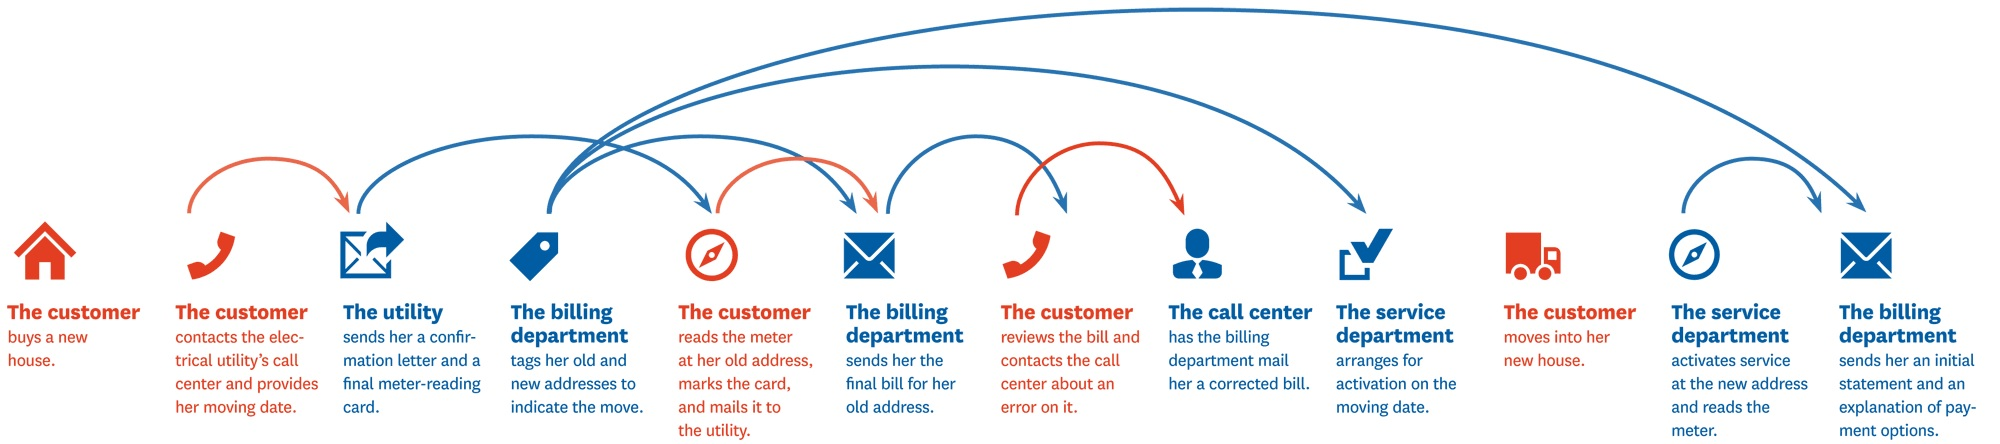
\includegraphics[width=\columnwidth]{example.jpg}
  \caption{Customer Experience Journey Touchpoints}\label{f:Customer Experience Journey}
\end{figure}

However, not all touchpoints are created equal \cite{Meyer2007}. There are some touchpoints that every customer may have to go through to get to the next step in the process and others that will produce a more valuable action, such as a purchase \cite{Meyer2007}. There are further questions today that did not exist in years past due to the advances in technology and how that affects customer behavior \cite{Kannan2017}. These advances in technology not only could influence customer behavior but also provide companies direction on which products they should produce, where these products should be placed, what price point is most optimal and how should they properly promote a particular product to their audience \cite{Kannan2017}. Big data and analytics can provide opportunity to inform the promotional piece as companies have utilized this feature to provide personalized and relevant content along  the customer journey as defined in figure \ref{f:Customer Journey} \cite{Stoicescu2015}. 

\begin{figure}[ht!]
  \centering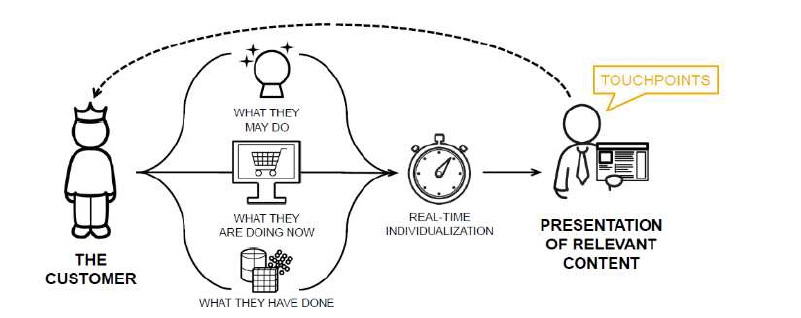
\includegraphics[width=\columnwidth]{customerjourney.jpg}
  \caption{Customer Experience Journey}\label{f:Customer Journey}
\end{figure}

While traditional advertising and marketing methods have included outdoor, print, television, and radio, among others, there is a growing shift in reaching customers via the digital space \cite{Kannan2017}. As of 2016, digital advertising spend reached 72 billion dollars, a 20\% increase from the year prior and now accounting for a third of all advertising revenue spent in the United States \cite{Center2017}. With the increased move to digital from more traditional outreach methods, the customer relationship is also being managed via digital platforms such as email, social, and mobile \cite{Kannan2017}. A customer's \textit{digital journey} can provide opportunities for big data and analytics to better understand the touchpoints along the way as well as where a company may be able to \textit{nudge} a customer appropriately to make a purchase decision. 

The objective of this work is to provide a view into the customer experience journey as it relates to big data and analytics. This overview of existing work is to allow one to see how a company or industry may start to match their big data efforts with the purchase decision that customers make as well as the multiple touchpoints included along the way. The move towards digital outreach and marketing efforts will also be defined to ensure the reader understands what is meant throughout as it relates to outreach and personalization efforts. Rather than the analysis of a specific dataset, real-world examples will be showcased across a variety of industries to provide detail as to how big data is being used to better understand the customer and enhance the journey they go through along the way. Lastly, this work will highlight the need of matching big data with the customer experience journey, challenges with pursuing this work going forward, along with recommendations on how to overcome these challenges. 

\section{What is the Customer Experience Journey?}
The way \textit{customer experience journey} is defined can differ by industry, product, and even by place. While past work has defined the customer experience journey as the process of purchasing a product or service, in today's landscape, it has become more than that. The Harvard Business Review would define the customer experience journey as the ``sum-totality of how customers engage with your company or brand, not just in a snapshot of time, but throughout the entire arc of being a customer" \cite{Richardson2010}. Traditionally, the customer experience journey and buying process were used interchangeably where a customer moves through a decision making process. Some key areas that were highlighted in a typical customer experience journey include: 

\begin{itemize}
    \item \textbf{Need Identification}: At this stage, this is where the customer decides whether they have a particular need that they believe the product or service could fill. There are times where properly identifying the need or problem can be an area of opportunity for a company \cite{DeAsi2017}. 
  \item \textbf{Awareness}: In order for customers to even engage with a product or brand, they first need to be aware that it exists. Further, the customer has to decide whether the product, service, or brand is relevant to them \cite{DeAsi2017}.
  \item \textbf{Evaluation of Alternatives}: Here, a customer starts to investigate the options available and educate themselves on the benefits and drawbacks of each. This is an area where companies seek to differentiate themselves from competitors as customers go through this stage in the progress \cite{DeAsi2017}. As customers continue in their research state, they can be influenced in a variety of ways such as through advertising and marketing, word-of-mouth or reviews from others, in addition to information they obtain in other ways through their own search process \cite{Kannan2017}. 
   \item \textbf{Purchase}: After a customer has gone through their choices to the best of their satisfaction, they move to the stage where they decide to make (or not make) a purchase \cite{Kannan2017}. 
    \item \textbf{Post-Action Evaluation}: After a decision is made, one way or the other, this is place where the consumer evaluates their decision which may include key questions such as \cite{DeAsi2017}: 
    \begin{itemize}
    \item Were my needs adequately met? 
    \item Am I satisfied with my choice? 
    \item If given the same circumstances, would I make the same choice again?
    \item Would I recommend the choice I made to others?
     \end{itemize}
\end{itemize} 

While the list of questions could be endless the intent is to move customers through this purchase decision process so companies create loyal customers and advocates \cite{Kannan2017}. However, that model is evolving with the shift to a multi-prong outreach approach via digital and non-digital methods \cite{DeAsi2017}. A longer customer experience journey is outlined in figure 1 as a customer can enter at any stage in the process. Pre and post purchase measures can be collected, stored, and analyzed at any point along the way as shown in figure \ref{f:Digital Marketing} \cite{DeAsi2017}. 

\begin{figure}[ht!]
  \centering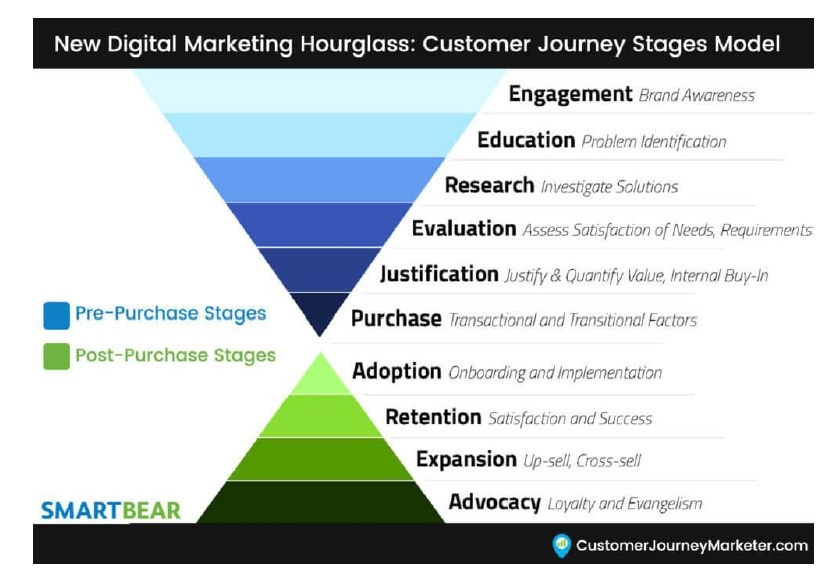
\includegraphics[width=\columnwidth]{digitalmarketing.jpg}
  \caption{Digital Marketing Customer Stages Model}\label{f:Digital Marketing}
\end{figure}

\section{What Does Digital Mean?}
With the influx of big data, analytics, and technology, there is often a rallying cry among leadership teams for an effort to be more \textit{digital}. However, when exploring the definition of \textit{digital}, it can greatly differ by audience, industry, and objective. Even within a singular company, alignment on what digital means can vary. Instead of trying to decide what digital \textit{is}, it may be more beneficial to think of what digital can \textit{do}. McKinsey highlights that digital should create value of some kind and offers various ways in which this can apply to an organization \cite{Dorner2015}. Despite varying definitions, methods, and applications of what digital is (and is not), there are commonalities in digital efforts that can be used to better understand this environment \cite{Hmeid2017}:
\begin{itemize}
  \item \textbf{Customer-Centric}: Digital efforts entail putting the customer first as they examine data and processes to enrich the customer experience \cite{Hmeid2017}. 
  \item \textbf{Real-Time}: Long gone are lag times between collecting, analyzing, and processing data to decision-making. Now, data collection is always on and can be pulled at any time \cite{Hmeid2017}. 
  \item \textbf{Connected}: With the volume, veracity, variety, and velocity of big data alone, the ability to have data sources and storage systems \text{talk} to one another is crucial to develop meaningful insights and inform decision making appropriately and effectively \cite{Accenture2013}. This not only has to happen from a technology standpoint but also from a company culture standpoint as well to ensure appropriate units and individuals are also talking to one another to better understand the customer experience journey overall. 
\end{itemize} 
It's important to note that while \textit{digital} can mean \textit{online}, one should not assume that these actions and behaviors only occur in the online environment. However, the collection, storing, and analyzing or these behaviors can be \textit{digital} or \textit{online} even though they may be reflective of what is happening in an \textit{off-line} setting. Overall, implementing digital capabilities should improve business processes, challenge new ways of thinking, and deliver ways to enhance the customer experience journey \cite{Accenture2013}. 

\section{What is Digital Marketing?}
While advertising and marketing methods go as far back as the 1800s where customer lists were used to determine how individuals could be influenced via direct mailing efforts, digital marketing has only come to be with the creation of the internet \cite{Couldry2014}. The internet has created opportunity for brands to directly connect with customers and likewise, for customers to engage with brands in a myriad of ways in the digital space \cite{Edelman2010}. While varying definitions of digital marketing exist, it is often categorized as a subset of traditional marketing where the ``use of digital technologies create an integrated, targeted, and measurable communication" to not only attract potential customers but engage with current ones for retention and loyalty purposes \cite{Grishikashvili2014}. Digital marketing became even more prevalent in the 2000s as companies such as Google, Yahoo, and Facebook provided opportunity to deliver ads at an individual level based on demographic and behavioral characteristics \cite{Couldry2014}. Other data collection firms offered the ability to track users across the web space to see which pages were viewed, clicked, and time explored to help further understand the experience of a customer across the web space \cite{Couldry2014}. With these advances in technology and understanding, the customer experience journey began to also transform along with the changes in advertising from traditional to more digital.

\section{How is Big Data Involved in the Customer Experience Journey and Digital Marketing?}
As the typical customer experience journey moves away from a traditional linear process and more towards an iterative approach, there is a need to understand the pathway among customers with data \cite{Edelman2010}. As of 2016, there are now approximately 3.7 billion individual users on the internet \cite{Akter2016}. This population size coupled with the multiple methods of interaction present an opportunity for companies to better understand potential customers in an effort to deliver the right message, to the right person, at the right time. A Gartner report states that the amount of data companies are collecting is growing by nearly 40 percent year-after-year \cite{Liyakasa2013}. Nearly one of out of every four state that there is a need to tie big data back to marketing-related efforts \cite{Liyakasa2013}. At the time of the report, it was estimated that only three percent of companies surveyed had a dedicated individual responsible for big data analytics and customer intelligence insight \cite{Liyakasa2013}. As the touchpoints with customers increase and also move more towards digital, so does the ability to collect and track the data from these touchpoints to better understand the customer experience journey \cite{Edelman2010}. 
\par 
One could argue that marketing data has been \textit{big} for quite some time given the sheer number of people exposed to efforts typically exceeds millions \cite{Couldry2014}. However, what has changed in this space is marketing's increased use of digital technologies to reach potential customers in the digital landscape across various channels including search, display, social media, email, etc. \cite{Kannan2017}. For companies to be successful in utilizing big data to inform digital marketing efforts and to better track and enhance the customer experience journey, incorporating the necessary technologies and talent is a must along with shifting the organizational culture to making data driven decisions \cite{Grishikashvili2014}. This process can be difficult as an individual user alone can generate ``billions of data signals" and attempting to understand which ones may be tied directly to a product or brand's marketing efforts can be a daunting and overwhelming task \cite{Couldry2014}. However, there are a few well-known companies that have started the shift in tracking the customer experience journey through big data analytics and applications. We will examine key industries that have leveraged this knowledge and insight to better understand and enhance their relationship with customers. 

\section{Big Data In Online Retail}
Companies like Amazon and eBay are often cited as pioneers in utilizing big data analytics considering these were companies that were \textit{born digital} \cite{Akter2016}. While other retail companies have made their way into the big data analytics environment, often times they are brick-and-mortar establishments in addition to offering electronic commerce (e-commerce) capabilities, such as Target, Sears, or Wal-Mart. Growth in e-commerce has taken place around the world with nearly 1.3 billion customers in existence as of 2016 \cite{Akter2016}. In the online space, there are multiple opportunities for these companies to track the customer experience from number of visits, keywords used in search, orders and products placed, frequency of purchases, in addition to when items in their virtual cart are abandoned or even when items are returned or complaints are filed \cite{Akter2016}. Amazon and eBay, among others, have utilized big data analytics to their advantage to create recommendations for their customers, develop predictive models, and also offer real-time changes in the customer's experience journey. 

  \subsection{How Does Amazon Use Big Data?}
  In 1995, Amazon started its life in the online space as an electronic bookstore \cite{Hartmans2017}. While early sales were still impressive totaling nearly \$20,000 a week, during their popular campaign of \textit{Prime Day} in 2017, analysts estimated that sales for that one day alone to be around \$500 million \cite{Smith2017}. As of July 2017, Amazon has approximately 300 million users with nearly eight out of ten that make a purchase at least once a month \cite{Smith2017}. The amount of information tracked per user continues to increase at an exponential rate as Amazon's growth has moved beyond their days of an online bookstore and into the realm of an \textit{everything} store, including acquiring other large companies such as Whole Foods \cite{Petro2017}. With this, there are a number of ways that Amazon uses big data to enhance the customer experience:
  
\begin{itemize}
 \item \textbf{Personalized Recommendations and Predictive Modeling}: As customers are exploring products on Amazon, they are often shown other suggested products either based on their own past purchase behavior or by what others who purchase similar items also bought \cite{Akter2016}. These recommendations are shown in real-time, often on the same web pages as customers are exploring other products \cite{Akter2016}. It is estimated that based on this ability alone, utilizing both structured and unstructured data, that 35\% of all sales are attributed to the recommendation algorithm, which would show that their predictive efforts are meeting the needs of their customers \cite{Akter2016}.  
 
 \item \textbf{Efficient Delivery}: Even though Amazon utilizes and houses large amounts of data about its customers to offer personalized recommendations and offers, the company also has to maintain a tremendous amount of data about its own operations to inform logistics and supply chain management to meet customer expectations \cite{Akter2016}. A key selling message of Amazon is delivering product in two business days, even in some cases offering same day delivery on certain items if they are ordered within a certain timeframe CITE[21]. With the increase number of products, suppliers, and customers, Amazon is still able to rely on big data analysis to maintain a consistent experience that doesn't compromise delivery for the customer which in turn leads to a better customer experience overall \cite{Akter2016}. 
 
 \end{itemize}

  \subsection{How Does eBay Use Big Data?}
  eBay is a website that also started in 1995 which offered a unique opportunity to bring together buyers and sellers in the online space \cite{Ebay2017}. Sellers could place their items online where buyers could potentially place bids, similar to if they participated in a live auction, where the item may go to the highest bidder. This allowed for others around the globe to connect and purchase items directly from another person while paying for the item through online methods. It is estimated today that there are nearly 180 million buyers and sellers and nearly 250 million search inquiries made per day on eBay \cite{Lui2012}. Like Amazon, eBay seeks to understand and tailor the online experience for customers through the use of big data in a multitude of ways as eBay itself states ``understanding the customer is key" \cite{Sararn2014}. Various methods utilized to better understand and tailor the customer experience journey include:
  
 \begin{itemize}
 \item \textbf{Web Page Metrics to Inform Layout}: It is estimated that among eBay customers, there is ``100 million hours of interactions collected per month" \cite{Sararn2014}. Through an extensive number of experiments and A/B testing, eBay is able to optimize the web experience for customers. From their big data analytics, they can find preferred layouts of web pages which can customize anything from navigation feature to the size of photos displayed on the screen \cite{Akter2016}.   
 
 \item \textbf{Ease of Finding Items}: Buyers and sellers alike utilize the search feature provided on the eBay website to find necessary items or to compare price points of like items when deciding which price point to utilize \cite{Lui2012}. Behavior patterns of customers have been used to inform how to best optimize the search feature in an effort to get customers to the necessary items more quickly which in turn will, hopefully, produce a sale \cite{Lui2012}. While in the past, the search algorithm would have taken words and terms in a more literal sense, though optimization eBay has been able to make the search algorithm more intuitive which has lead to more sales \cite{Lui2012}. Such examples show that originally when customers would shorten words used in the search feature, they may not find what they need. However, after analysis of customer inputs and changes in the search algorithm, this ability was taken into account so customers could still find the necessary product without changing their behavior. 
 
 \end{itemize}
 
\section{Big Data in the Finance Industry}
There are a number of products and services available in the finance industry ranging from personal and business loans, to stocks, retirement accounts, and credit cards. Companies such as JP Chase Morgan, American Express, and Bank of America are capitalizing on big data use to inform their offerings and also better understand their customer base \cite{Woodie2016}. These companies are monitoring the customer experience journey through all touchpoints which could include web visits, phone calls, and even in-person interactions \cite{Groenfeldt2012}. This information can also be used to detect fraud on certain accounts when activity occurs that may not be typical of their customer \cite{Woodie2016}. These algorithms and techniques can in turn ensure customers are protected which help with customer retention. Conversely, those in the finance industry may also be able to utilize big data and mining techniques to determine if they are about to lose a customer. One such company that utilized these methods to their advantage is American Express, which accounts for nearly a quarter of all credit cards transactions and totals more than \$1 trillion annually in customer purchases \cite{Morgan2014}. 

  \subsection{How Does American Express Use Big Data?}
  In 2010, American Express invested in big data technologies and resources, including Hadoop, to increase capabilities to detect fraud, provide recommendations to current customers, predict who may close their accounts, as well as acquire new customers \cite{Woodie2016}. These methods are used to assist in efforts to maximize the customer experience journey through the use of:
  
 \begin{itemize}
 \item \textbf{Fraud Detection}: To minimize loss, fraud alerts have to happen quickly. To achieve this, American Express implemented machine learning algorithm techniques \cite{Manglani2017}. Data points included in the model consisted of information about the merchant where the purchase occurred, purchase details such as items bought and price, and even customer information \cite{Manglani2017}. By analyzing patterns in real-time, American Express was able to flag possible fraudulent activity in a matter of milliseconds which then allows the company and customers more time to prevent further loss with the increased capability \cite{Manglani2017}. American Express was able to identify an additional \$2 billion in fraudulent activity that that they were not able to identify before and therefore protect their customers and ensure a more positive customer experience as a result \cite{Manglani2017}.  
 
 \item \textbf{Personalized Recommendations}: Along with protecting their customers, American Express also seeks to understand how to better engage their customers through personalized recommendations. One such example is based on analyzing customers past transactions along with geographic location information to push specific recommendations to customers in real-time \cite{Woodie2016}. Through the use of big data analytics, the company can send recommendations on similar restaurants in the area if they see from a customer's transactions they frequent a certain genre or area \cite{Woodie2016}. These recommendations also work on behalf of the merchants who accept American Express as the company can provide information on purchases in the area which merchants can use to create offers to entice customers to purchase products and services by using their American Express card at their particular store \cite{Economist2016}.  
 
  \item \textbf{Churn Prediction Models}: American Express also uses its vast amounts of data to see if they can predict whether a customer will close their account \cite{Manglani2017}. By incorporating machine learning models, they can better understand the customer experience and appropriately jump in at different points along the journey in an effort to deter customers from closing their accounts. Through analysis of past transactions as well as nearly 100 other variables incorporated to understand customers, the company estimated that for one model, they were able to identify nearly one out of every four accounts they believed would have closed in the near future \cite{Manglani2017}. With this information, tailored marketing and messaging could be implemented to help with retention rates. 
 
 
  \item \textbf{Acquiring New Customers}: Despite the large base of customers, merchants, and transactions, there is always a need for businesses to grow to increase revenue and capabilities for the future. One way to achieve this is through digital marketing efforts targeted at those who may be potential customers for American Express. Through their efforts, American Express was able to grow their customer base by nearly 40\% through online marketing efforts \cite{Manglani2017}. With these more targeted and cost-effective measures, American Express was able to efficiently acquire new customers as compared to more traditional marketing efforts of the past, such as direct mail \cite{Manglani2017}. These optimizations further enhance the customer experience journey by delivering them a message at the right time through the right medium. 
 \end{itemize}
  
\subsection{How Does Bank of America Use Big Data?}
While big data, analytics, and predictive models can be used to better understand how to reach out, retain, and attract customers, these same techniques can be applied when determining how to optimize the customer experience journey from an internal perspective. Considering the journey can take place across a series of touchpoints, Bank of America was one major bank, among others, that utilized big data to better understand how to better serve their nearly 50 million customers \cite{Davenport2013}. One method included:

 \begin{itemize}
 \item \textbf{Customer Segmentation}: Through the use of big data, Bank of America acknowledged that their customer base could be divided into segments and therefore their behavior and needs differed \cite{Davenport2013}. By analyzing online correspondence, calls from a call center, and even visits to area braches, appropriate offers could be tailored to the customer \cite{Davenport2013}. Utilizing data points provided in the online space along with the ones that occurred elsewhere, a new program was developed by Bank of America \cite{Davenport2013}. With this new program and customized offerings, customers were more highly engaged with by Bank of America which increased customer satisfaction and experience as a result \cite{Davenport2013}.  
  \end{itemize}
  
\section{Big Data in the Healthcare Industry}
Rising patient volumes, increasing aging population, and mounting costs have all contributed to the growth, importance, and complexity of the healthcare industry \cite{Nambiar2013}. As of 2016, it is estimated that nearly \$4.1 trillion will be spent on healthcare costs in the United States alone \cite{Nambiar2013}. Nearly 290 million people in the United States have some form of insurance or healthcare coverage but that also leaves nearly 28 million who are uninsured \cite{Foundation2016}. A typical customer can interact with a number of stakeholders throughout their healthcare journey ranging anywhere from their initial doctor's visit, to filling a prescription at the pharmacy, to paying a bill to their insurance provider. One may then ask based on these interactions: how does the online space play into the healthcare industry at all?

With the move to electronic medical records (EMR), the ability to now aggregate years of information on an individual, as well as an entire population, becomes more of a reality \cite{Froves2013}. Even though the healthcare industry has lagged behind other industries regarding their collection and use of big data, they are one of the most important as it relates to utilizing their information to create a better experience for customers as it pertains to the their health \cite{Froves2013}. The ability to link this data across various stakeholders is also critical in understanding the full journey of a customer (or patient) to ensure effective treatment decisions are made. Health Information Exchanges (HIEs) allow for this opportunity and the HIE has information on more than 10 million patients, over a span of nearly 80 connected hospitals, and approximately 18,000 physicians have access \cite{Froves2013}. Big data in the realm of healthcare provides tremendous opportunity to create value for customers and healthcare professionals alike. One such software company explored this use of connected data sources to better inform healthcare providers with practice-based evidence in an effort to tailor care for an individual patient \cite{Central2017}.

\subsection{How Does Apixio Use Big Data?}
As others have stated about healthcare related data and reporting, ``the problem in healthcare is not lack of data, but the unstructured nature of its data" \cite{Marr2016b}. Apixio, a cognitive computing firm based in California, wanted to take on the challenge of making unstructured healthcare related data available and easier to use in order to better aid decision making in patient treatment \cite{Marr2016b}. Their work involved taking clinical charts of patients and combining them with notes from physicians, test results, and even hospital stays to develop a more complete picture about an individual \cite{Marr2016b}. From there, Apixio was able to provide benefits based on this big data process:
 \begin{itemize}
 \item \textbf{Patient Model Development}: Data at an individual level was used to develop patient models from a series of text processing and coded healthcare data \cite{Marr2016b}. By creating a profile per individual, like individuals could then be grouped together which in turn helped to inform what treatments or procedures would work best in those individuals who fit a certain criteria \cite{Marr2016b}. Considering this information is derived from actual practice of medicine, it can better inform clinical care and also ensure that patients are set up for best optimal outcomes if treatment decisions are made based on big data collection and analysis \cite{Marr2016b}. 
  \item \textbf{Healthcare Cost Savings}: Cost of healthcare continues to be a growing concern for both customers and other key players such as healthcare professionals and insurance companies \cite{Nambiar2013}. With the move to EMR and big data analytics, it is estimated that anywhere between \$300 and \$450 billion dollars can be saved in healthcare costs \cite{Nambiar2013}. With the use of big data technology and methods, Apixio developed a system that could read and code patient chart information \cite{Marr2016b}. Typically, this method of coding would have been performed manually by a person or set of individuals, and with that comes a laborious and expensive process \cite{Marr2016b}. Apixio's capabilities were also found to be more accurate resulting in 20\% improvement in accuracy which in turn lead to better decision making among healthcare providers \cite{Marr2016b}. The also helped individual customer to ensure they were getting billed appropriately for the right treatment or procedure as well as for the insurance company who may be providing coverage \cite{Marr2016b}. These techniques then allow for an improved customer experience journey if costs can be mitigated through the use of big data initiatives that allow for better efficiency and accuracy. 
  \end{itemize}
 \section{Big Data in the Entertainment Industry}
The entertainment industry includes a wide array of forms including newspapers, movies, books, television programs, and radio \cite{Griffith2017}. As of 2016 it is estimated that this industry is worth approximately 1.8 trillion dollars in the United States alone \cite{Statista2017}. Streaming video services such as Netflix and Hulu have entered the market in recent years and provide a further opportunity to deliver content directly to customers. As of 2016, video streaming services are the second largest category for home entertainment with customers in the United States spending \$6.2 billion \cite{Atkinson2016}. The wealth of data collected from these streaming services include but are not limited to the type of content watched, when content is watched and on which type of device, as well as how often it takes for customers to make a selection down to an individual user level \cite{Cohen2017}. Netflix is one of the many video streaming leaders and has made big data and analytics a foundation to their business strategy and outreach initiatives \cite{Jenkins2016}. 

\subsection{How Does Netflix Use Big Data?}
While Netflix once started out as a mail-subscription video rental service, the business model has shifted to provide content entirely online and caters to nearly 60 million subscribers in over 50 countries \cite{Jenkins2016}. Netflix's competitive advantage in the market place stems from their ability to use big data as they estimate that they process over 10 petabytes of data a day which includes more than 400 billion new events \cite{Jenkins2016}. Utilizing programs and data scientists, Netflix began to seek out additional opportunities to understand customer preferences and to also optimize the experience journey through a variety of different methods: 
 \begin{itemize}
    \item \textbf{Personalized Recommendations}: Netflix not only analyzes what a particular person may watch but also what others who \textit{look like} that user may enjoy based on data such as age, gender, or even zip code \cite{Jenkins2016}. With the sophistication of the recommendation algorithm, viewers spend an average of 17.8 minutes browsing through the selections before picking a program to watch       \cite{Jenkins2016}. Spending more time increases the level of engagement with users and also extends the lifetime value of the customer in an effort to help with retention \cite{Cohen2017}. By delivering relevant content, Netflix estimates they save more than \$1 billion per year by their efforts in keeping customers happy \cite{Cohen2017}. 
    \item \textbf{User Choice}: In addition to providing the right recommendations, ensuring that the image or artwork for films is appropriate to the user also aids in choice \cite{Cohen2017}. Netflix engages in A/B testing of program thumbnails images and also seeks out feedback from users on which images they prefer \cite{Cohen2017}. From this process, Netflix was able to increase video viewing between 20-30\% when utilizing the right images and listening to customers' preferences \cite{Cohen2017}. 
    \item \textbf{Customized Content}: Analyzing what audiences enjoy watching can provide insight as Netflix sought to create their own content \cite{Jenkins2016}. One common cited example includes the development of \textit{House of Cards} as an original Netflix series that was created with big data information \cite{Jenkins2016}. Netflix found that the original series from the British Broadcasting Corporation (BBC) did well with audiences and that Kevin Spacey movies were also popular \cite{Jenkins2016}. Further using customer data, Netflix understood that customers \textit{binge-watched} seasons of shows and therefore releasing an entire season at a time would best meet the needs of their customers versus one episode at a time \cite{Jenkins2016}. The year the \textit{House of Cards} series premiered, subscribers grew from 27.1 to 33.4 million and the show received countless Emmy and Golden Globe nominations and awards \cite{Jenkins2016}. By utilizing big data, Netflix was able to create and deliver content that customers wanted and also help their bottom line \cite{Jenkins2016}. 
\end{itemize}

\section{Big Data in the Gaming Industry}
In addition to the entertainment economy, the gaming sector also is substantial in size and revenue. In 2016, the commercial gaming industry grew to \$38.7 billion across 24 states and nearly 600 casinos \cite{Rubinrown2017}. Las Vegas, a leader and popular gaming destination had a record year of visitors at nearly 43 million \cite{Rubinrown2017}. With increased competition among entertainment resorts and casinos in Las Vegas, as well as other parts of the United States, the need to create an optimal customer experience is crucial to attract customers and also keep them engaged. Metro-Goldwyn-Mayer (MGM) Resorts International and Caesars Entertainment are two conglomerates that have capitalized on big data use to better tailor the customer experience journey. 
\subsection{How Does Caesars Entertainment Use Big Data?}
Caesars has described their customer relationship optimization process as utilizing a ``data-driven and closed loop approached to deliver a personalized experience" \cite{Welch2012}. A few ways they have implemented this include:

\begin{itemize}
 \item \textbf{Creating Customer Loyalty}: Demographic, gameplay, and other transactional data is kept on each guest to create a detailed profile \cite{Welch2012}. Employees then across the establishment can utilize this data to personalize offerings and incentives to customers, anywhere from how he or she is greeted by staff to whether complementary services should be offered to improve the customer experience \cite{Welch2012}. This type of treatment isn't just limited to \text{big spenders} at the casino but translates across all customers in an effort to create loyalty across multiple segments \cite{Welch2012}. 
 \item \textbf{Efficiencies Through Mobile Application}: Caesars also offers guest the ability to utilize their mobile device to conduct tasks such as checking into to a property or even ordering a drink from the bar to avoid long lines \cite{Welch2012}. Incentives can also be pushed directly to customers based on their location and preferences such as tickets for shows or dining options in the area \cite{Welch2012}. Considering most guests carry their phone in their pocket, engaging with them on the casino floor can create a better customer experience to give them what they need, when they need it \cite{Welch2012}. 
\item \textbf{Customized Experiences}: The vast amounts of data collected on customer behavioral patterns in terms of which machines are played, when, where, and by whom can provide insight into how to best tailor offerings \cite{Schull2012}. For example, it was observed that an elderly population visits the casino at a certain time of day and therefore with the influx of that audience, casinos are able to adjust game offerings in real-time offering enlarged text for better viewing among the visually impaired in that age group as well as bet levels for certain games \cite{Schull2012}. By analyzing heat maps of popular games and parts of the casino, it also allows for companies to staff appropriately to ensure customer needs are being met based on predicted demand \cite{Schull2012}. These real-time changes enhance the customer experience journey by tailoring offerings to specific customer segments. 
\end{itemize}
\subsection{How Does MGM use Big Data?}
Similar to other casinos and resorts, MGM has utilized past customer data in an effort to better predict future behavior \cite{Nair2016}. However, they have also utilized this data to create personalized marketing offers to entice frequent (and non-frequent) visitors back into the experience \cite{Nair2016}. Though sophisticated modeling efforts, MGM is able to tailor marketing efforts to include a variety of different incentive types and levels. The final result of this process created 120 models of customer behavior with approximately 180 variables in each as well as 20,000 parameters across all which showcased an increase in revenue at a lower cost \cite{Nair2016}. These models were used to inform marketing efforts across a variety of areas, including but not limited to \cite{Nair2016}: 

\begin{itemize}
 \item \textbf{Hotel Room Rates}: Attributes such as room type, discount, number of times, etc., all play a role in which aspect will draw a customer back into the establishment \cite{Nair2016}.  
 \item \textbf{Entertainment Add-Ons}: Type of entertainment offered, ticket price, or even facility features were all used as inputs in the model \cite{Nair2016}. 
\item \textbf{Other Offers}: Air packages, limo rides, resort credits, and many others were also used as way to determine which customers would respond to which offers \cite{Nair2016}. 
\end{itemize}

\section{Big Data in the Transportation Industry}
Whether by plane, train, car, or other means, today's American customer relies on some sort of transportation to get them to varying destinations whether it be work, school, or even vacation. An average person spends 20\% more time commuting today than they did 30 years ago \cite{Clifford2017}. With this come questions to the transportation industry as to where they should expand highways, add public transit, or open additional hubs or destinations for travel. Big data can be one avenue in exploring and answering these questions as well as create a more enjoyable experience for the customer if they can spend less of their life commuting. The introduction of the ride sharing mobile application of Uber also arose based on customer needs and preferences and through the use of big data is thriving as alternative transportation option \cite{Cohen2016}. Large airline carriers have made use of big data as they seek to understand buyer behavior so they can effectively plan flights and other amenities to meet customer needs \cite{Noyes2014}. 

\subsection{How Do Airlines Use Big Data?}
In just one day's time, it is estimated that there are nearly 42,000 commercial flights and 2.5 million passengers \cite{Administration2017}. From purchasing a ticket, to taking a flight, and (hopefully) receiving their checked baggage at their final destination, airlines collect a wealth of information on their customers throughout their flying experience \cite{Noyes2014}. When looking at key attributes that are analyzed and down to an individual level, airlines collect information about purchase history, arrival, departure cities, and dates, in-flight food choices, connecting cities, travel companions, as well as miles and credit card points earned and used \cite{Exastax2017}. While airlines have succeeded in collecting this data, using it to better enhance the customer experience journey is still a work in progress \cite{Noyes2014}. Those who work in the travel software environment and frequently provide products and services to those in the airline community to better understand their data even state they have ``not seen a single major airline with an integrated big data business solution" \cite{Noyes2014}. With that in mind, highlights from major airline players are explored even though full development of utilizing big data may still be on-going in this industry. 

\subsection{How Does Southwest Airlines Use Big Data?}
 One way that Southwest Airlines is utilizing big data is by trying to identify new opportunities for revenue \cite{Noyes2014}. By analyzing customer behavior online, Southwest is able to support their relationship with customers by offering the best rates in real-time \cite{Noyes2014}. They are also able to look at searches for destination pairs and make determinations on whether certain flights should be added to keep their customer base loyal and ultimately satisfied by getting to where they need to be, when they need to be there \cite{Exastax2017}. Not only is Southwest looking to meet the needs of customers as they make a flight choice, but they also seek to comprehend customer interaction at other points in the purchase process \cite{Exastax2017}. By utilizing a speech analytics tool, the company can better understand recorded conversations that take place with representatives as well as social media chatter \cite{Exastax2017}. These real-time insights can then inform customer service representatives as they interact with customers and guide them to deliver the optimal solution in various situations \cite{Exastax2017}. In addition to optimizing the customer experience from a satisfaction standpoint, Southwest airlines has also partnered with NASA on potential safety initiatives where machine learning algorithms can be used to spot potential abnormalities \cite{Exastax2017}. These efforts enhance the customer experience journey by not only looking out for safety of individuals but by also meeting their needs based on behavioral data. 

\subsection{How Does Delta Airlines Use Big Data?}
In a quest for customer loyalty, Delta Airlines has made an intentional effort in investing in their baggage tracking system to better meet customer needs \cite{School2015}. With this \$100 million dollar initiative, it not only gives airport operation teams the opportunity to identify trends in mishandled luggage situations but also real-time information to baggage handlers when transferring or sorting through bags \cite{School2015}. Similar information is also shared with travelers so they can track the progress of their bags down to the minute \cite{School2015}. With approximately 130 million bags checked in a given year on Delta Airlines, there is a common concern among customers on whether their bag will arrive at their final destination \cite{Noyes2014}. Giving customers a piece of mind allows for a more beneficial customer experience and also increases satisfaction and loyalty. The luggage tracking app has been downloaded 11 million times and has reduced the rate of mishandled luggage by nearly 71\% since 2007, which is better than any other airline \cite{School2015}. 

\subsection{How Does Uber Use Big Data?}
Founded in 2009, Uber started as a technology company and created a mobile application that connected those seeking transportation with those who were drivers \cite{Cohen2016}. Now, with nearly 8 million users who have connected with over 160,000 drivers, nearly half of the United States population has access to Uber in their city \cite{Institute2017}. The only opportunity to connect riders and drivers is through the mobile app consolidating data collection and tracking from the start; however, the sheer volume and real-time application of data use to inform pricing and availability still presents on-going challenges \cite{Cohen2016}. Demographics, frequency of trips, destinations, price, as well as sessions that do not end with a purchase are all recorded from the application \cite{Cohen2016}. Several ways in which Uber utilizes big data to meet customer needs includes:

\begin{itemize}
 \item \textbf{Matching Supply and Demand}: By analyzing travel transactions, Uber can appropriately plan for busy nights so customer travel needs are met \cite{Cohen2016}. Customers are also able to give feedback about their ride experience and rate drivers \cite{Central2017}. With this capability, the company can inspire trust and improve satisfaction if they find that certain drivers are not meeting expectations \cite{Central2017}. UberPool is also a new feature that has been added that allows for carpooling of customers where real-time analytics search for other customers in the area by geography \cite{Central2017}. This can therefore improve the customer experience for those who want to share a ride and split the cost appropriately \cite{Central2017}. 
 \item \textbf{Dynamic Pricing Model}: Uber is also able to adjust pricing models accordingly based on time of day \cite{Cohen2016}. Fair estimates are also able to be given in real-time which allow the customer to adjust their travel plans if needed and also pick the type of transportation, such as a sedan or sports-utility-vehicle (SUV) \cite{Cohen2016}. However, there are times that Uber uses these models to the company's advantage and offer \textit{surge} pricing in the events of heavy demand or traffic \cite{Cohen2016}. All financial transactions take place via the application with no exchange of cash. Pre-set and transparent pricing structures allow customers to select what fits their needs, even if they find their choice is to not take a ride at a particular time. Having the necessary and accurate information provided at time or purchase makes for a more enjoyable customer experience journey \cite{Central2017}.  
\end{itemize}

\section{Why is Using Big Data to Optimize Customer Experience Journey Important?}
These examples are a select few to showcase how companies can better understand and further the customer experience journey by leveraging big data. The average customer is presented with more choices today than ever before \cite{Meyer2007}. With this, companies today have to be more strategic to get the attention, time, and loyalty of customers to remain in the marketplace. Doing so can provide many advantages to both companies and customers as they utilize big data to better understand the customer experience. As Rawson et al state: ``companies that excel in delivering journeys tend to win in the market" \cite{Rawson2013}. Trends presented showcase how big data can provide big benefit:

\begin{itemize}
 \item \textbf{Retention of Customers}: It is estimated that ``acquiring a new customer can be between five and 25 times more expensive than retaining an existing one" \cite{Gallo2014}. Utilizing big data to predict when customers may close accounts can help to inform company efforts and ultimately prevent potential revenue loss if they can keep existing customers. American Express showed that by using big data and predictive analytics, the company could identify these customers sooner versus wait until the customer is already lost. 
 \item \textbf{Personalized Outreach}: Tailored communication messaging, and recommendations can give customers a better experience in getting what they need from companies but also benefit the company's bottom line as well. As Netflix and Amazon have showcased, providing recommendations to customers increases engagement and purchase behavior.  
 \item \textbf{Company Process Efficiencies}: Utilizing big data to understand customer behavior can help companies determine whether changes or improvements need to be made in how they deliver products and services to customers. As the Delta example showed, tracking baggage was not only a concern to customers but by doing so, the company improved their mishandled luggage rates. These efficiencies not only create satisfied, and possibly loyal, customers but also ensure that companies are spending their resources effectively by not making costly and time-consuming errors.  
\end{itemize}

\section{What Challenges Exist in Utilizing Big Data for the Customer Experience Journey?}
While big data use is going to be a crucial component going forward in understanding the customer experience journey, companies do face challenges in making this a reality, specifically:
\begin{itemize}
\item \textbf{Data Ownership} Customer data can live in a variety of places within one organization. The departments in which this data lives can be in silos with multiple departments not talking to one another or not willing to share what they feel their department owns \cite{Spiess2014}. 
\item \textbf{Company Culture} Cooperation across the organization can be a significant barrier in truly understanding the full customer experience. \cite{Spiess2014}.  
\item \textbf{Lack of Strategy} Without a clear strategy, it can also create issue in trying to determine how to best interpret and apply the findings in the data. This can lead to gaps in the organization if it is unclear what the ultimate goal is and which parties play a role \cite{Spiess2014}. 
\item \textbf{Resources and Skills} The technical aspects of understanding the customer experience journey can be a barrier as well. Having the right technology, people, and time in place to understand the full customer journey can also be a challenge for companies. \cite{Court2015}
\item \textbf{Consumer Behavior Volatility} Not all decisions made by customers are rational ones and there can be a variety of factors in play that big data can not track \cite{Stoicescu2015}. As further detailed in other work ``people do not behave like robots," so even when all the variables are optimized, outside forces beyond the control of a company could influence choice along with a customer's own emotions which big data doesn't always include \cite{Richardson2010}. 
\end{itemize}
Since within one company there can be different systems, different processes, and a variety of people employed with different skillsets, trying to address all of these challenges can be overwhelming. However, with challenges come opportunities and areas in which companies can focus on as they strive to have data that is connected, customer-centric, and available to look at in real-time \cite{Spiess2014}. 

\section{How Can a Company Overcome These Challenges?}
As companies seek to better understand their customer base through the use of big data and analytics, from the research performed, there are some steps that companies can take as they further explore opportunities to optimize the customer experience journey. Some key areas and questions to consider include:
\begin{itemize}
 \item \textbf{Seek to Understand Your Customer}: Big data and analytics can be a valuable starting point in understanding the pathway to purchase among your customers as well as which areas where you may be losing customers in the process. However, big data should be used in conjunction with small data as companies seek to understand the \textit{why} behind customer behavior. Gathering feedback from customers is essential in the process in optimizing their journey. 
 \item \textbf{Set Clear Objectives and Roles}: Given that earlier research highlighted that a very small percentage of companies have a dedicated person for customer analytics, first establishing a dedicated person or team could help in developing a better understanding of the data involved in tracking the customer experience journey \cite{Nichols2013}. This person or team of people can provide guidance to others within an organization by being a central source of knowledge about the customer. A key part of research is also setting clear questions and objectives at the beginning. Which data points are truly a part of the customer experience journey? What connections do we need to establish in order to move our strategy forward? How will we measure the return on our efforts?  
 \item \textbf{Make the Necessary Investment}: As other companies in this research highlighted, big data skillsets are necessary in understanding the customer experience journey which may mean a company may need to add data scientists, analysts, or other like positions within an organization. Additional technologies and tools may also be needed such as Hadoop or languages such as R or Python in an effort to process big data to derive insight. 
 \item \textbf{Test, Assess, and Optimize}: As companies look to establish dedicated resources, time, and people in the process of understanding the customer experience journey, there must also be acknowledgement that this process is iterative. There could be efforts that are not fruitful or plainly, do not work. However, as other companies have shown, the ability to test can provide this insight and allow the opportunity for a company to change course if needed.
\end{itemize}
While there are likely other areas to consider, this initial outline described can provide companies and those within an opportunity to start understanding the customer experience journey from a big data and analytics perspective. A company has to also prioritize these different efforts accordingly as it may not be possible to implement these changes at once. A company must also consider what their own \textit{success} will look like over time as progress is made.  

\section{Conclusion}
The customer experience journey will continue to evolve as new technologies are developed that can influence the multitude of touchpoints one experiences along the way as they make purchasing decisions. While big data and analytics can provide a picture as to what customers are doing, leveraging learnings from this work to better understand the customer experience journey will be key as competition in the marketplace continues to increase across a variety of industries. These examples show that by having the right tools, skillset, and objectives in place that utilizing big data to better meet the needs of customers can be successful. While the undertaking of this endeavor may not be quick or necessarily easy, it can provide great benefit to both companies and customers to deliver relevant products and services with the customer experience in mind.  Even though big data is a means of tracking the customer experience, big data is also changing the customer experience through digital marketing and outreach efforts in a way to effectively and efficiently engage and connect with customers. With this approach, the ability to deliver the right message, to the right person, at exactly the right time in the customer experience journey can provide tremendous opportunity for companies but also benefit the customers to have a more fulfilling experience journey with a company or brand. 

\begin{acks}

  The author would like to thank Dr. Gregor von Laszewski and the teaching assistants for their support and guidance in writing this paper in addition to the resources provided by the School of Informatics, Computing, and Engineering at Indiana University in Bloomington. 

\end{acks}


\bibliographystyle{ACM-Reference-Format}
\bibliography{report} 


\end{document}
